Ovo poglavlje če uključivati postavljanje VPN-a na FreeBSD inačici operacijskog
sustava BSD. 

\subsection{Postavljanje FreeBSD poslužitelja}
    Potreban nam je poslužitelj za po mogućnosti sa statičkom IP adresom. Ovdje
    ćemo koristiti platformu DigitalOcean koja omogućuje brzo i jednostavno
    podizanje i upravljanje poslužiteljem. Za pristup poslužitelju koristit ćemo
    ssh protokol za što nam je potreban par ključeva koje generiramo naredbom \\

    \noindent
    \code{\$ ssh-keygen -t rsa -b 2048} \\

    \noindent
    Javni ključ se nalazi u datoteci \code{~/.ssh/id\_rsa.pub}, a privatni, koji
    mora ostati tajan, u \code{~/.ssh/id\_rsa}.

    Nakon registracije na Digital Ocean na svojem profilu možemo dodati javni ključ
    koji ćemo kasnije koristiti za pristup poslužitelju. Sada možemo stvoriti
    poslužitelja. Odabrat ćemo opciju
    \textit{Create Droplet} i odabrati sljedeće postavke:

    \begin{figure}[h]
        \centering
        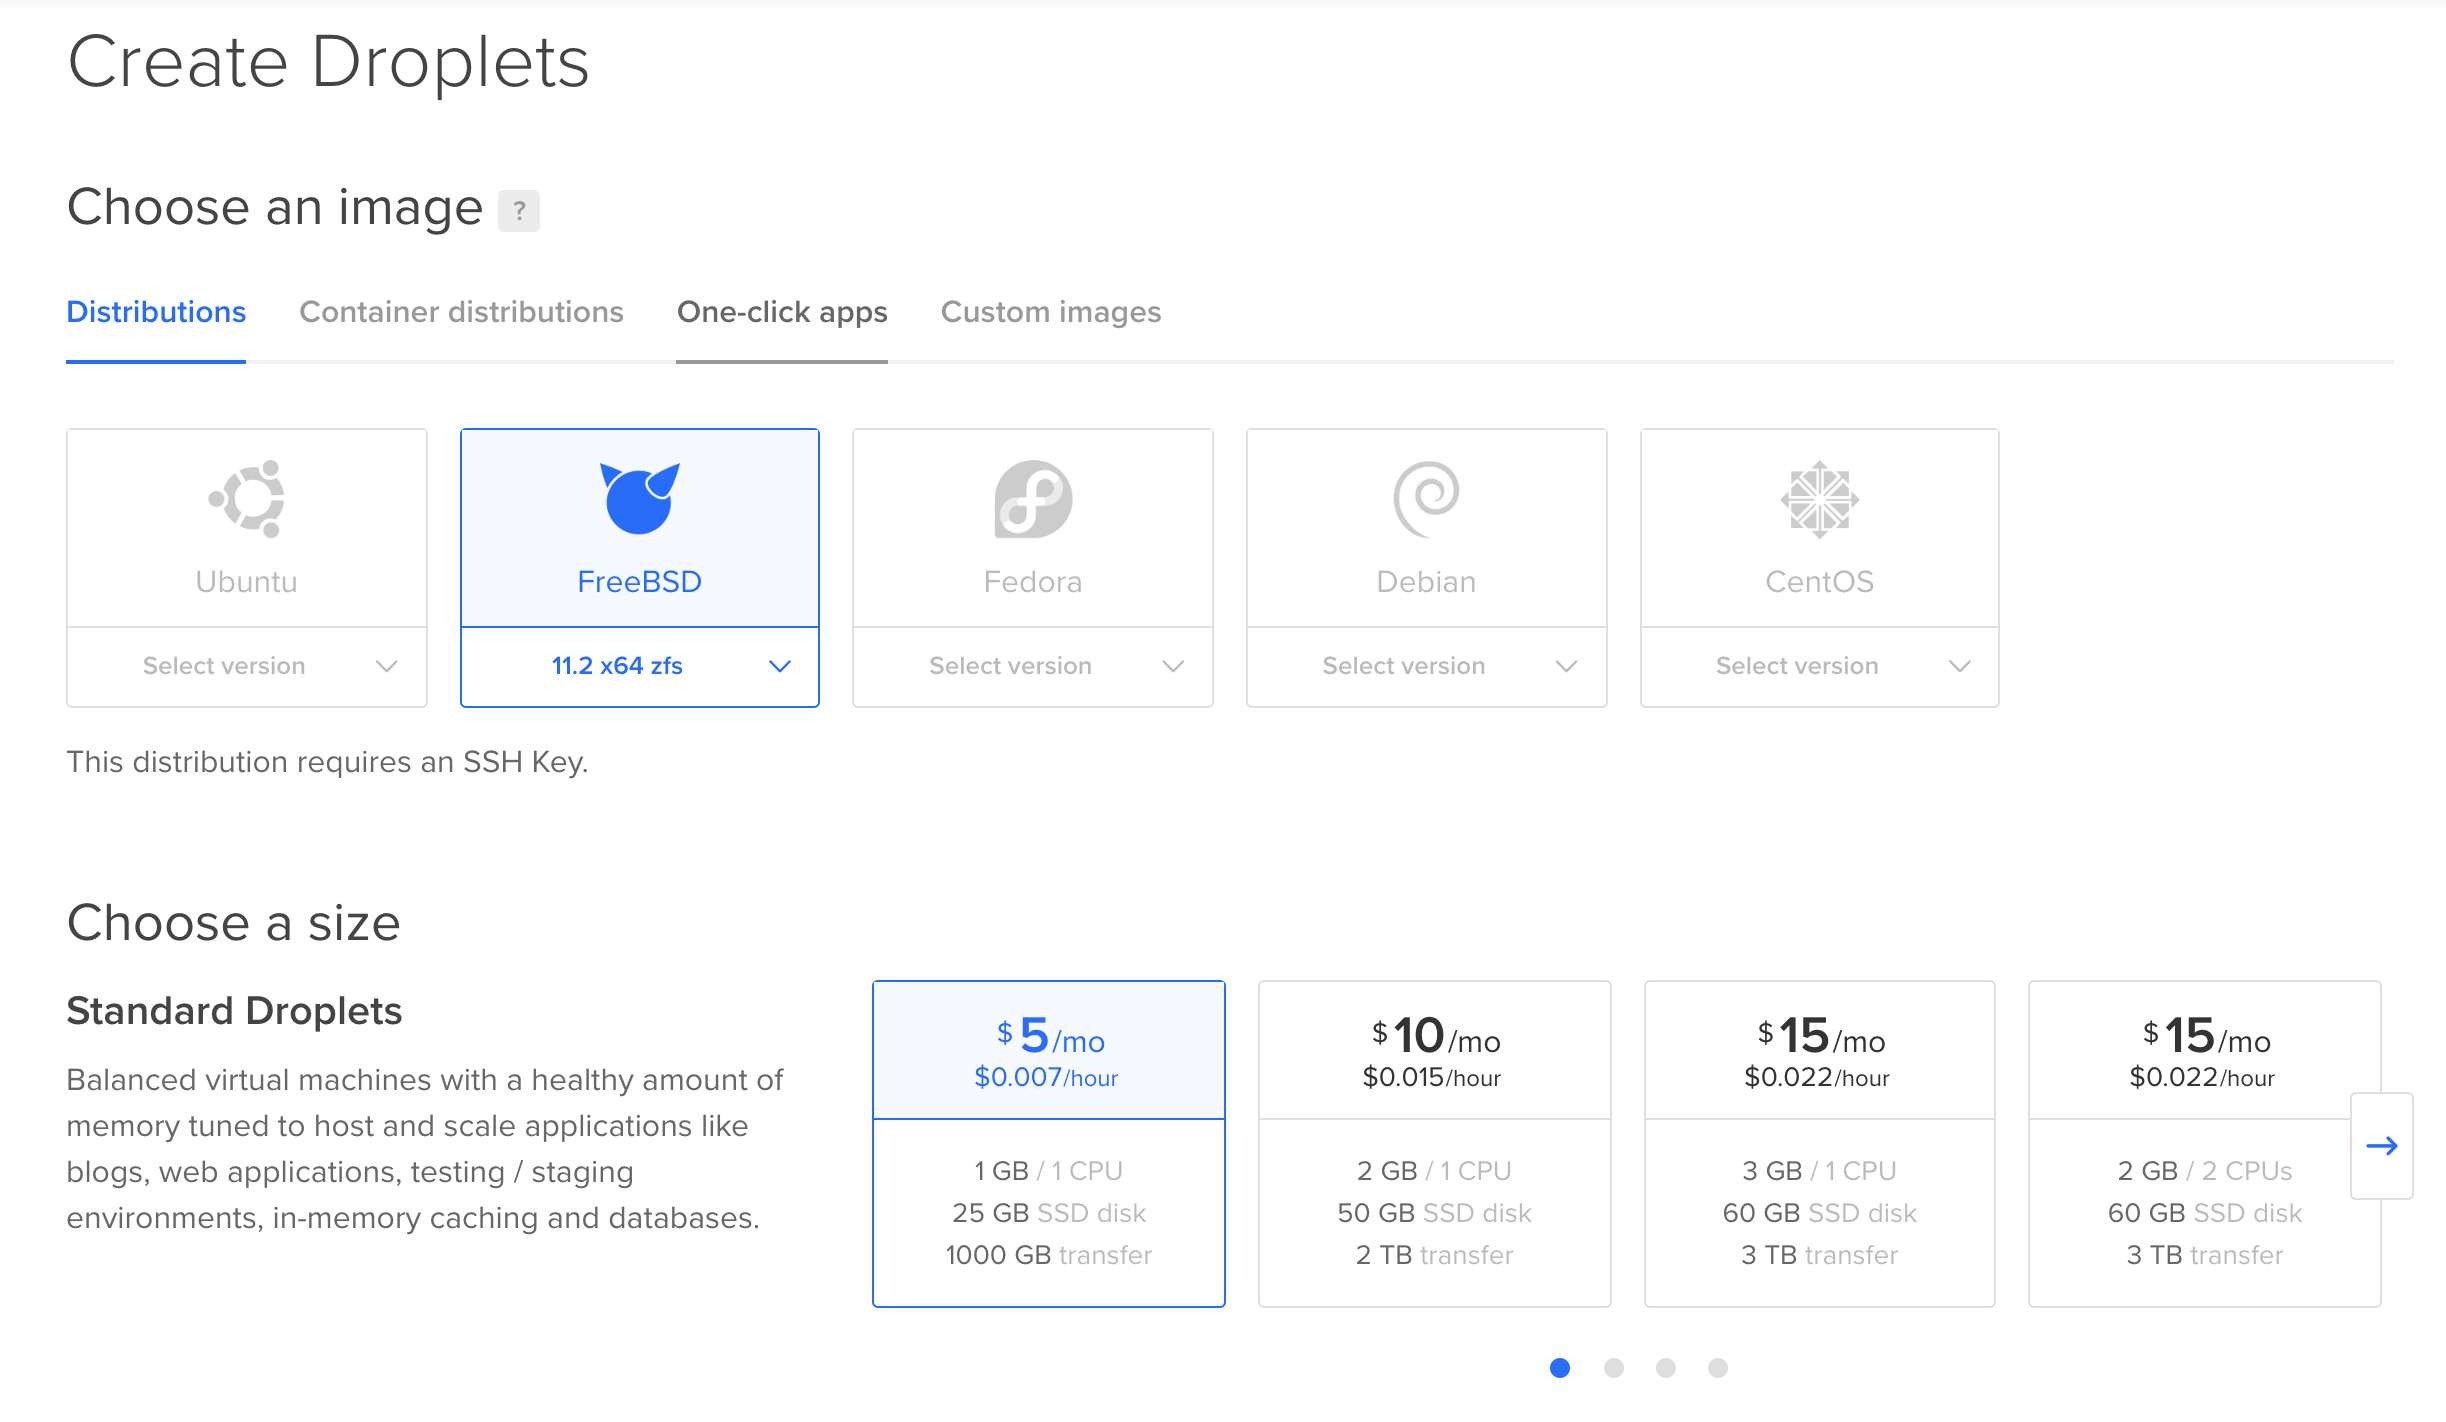
\includegraphics[scale=0.35]{slike/postavkeDOserver}
        \caption{Postavke DigitalOcean poslužitelja}
    \end{figure}

    \newpage
    \noindent
    Digitlal Ocean nam također nudi opciju da odaberemo lokaciju našeg poslužitelja
    i pripremimo ssh ključeve kako bi si olakšali pristup
    \begin{figure}[h]
        \centering
        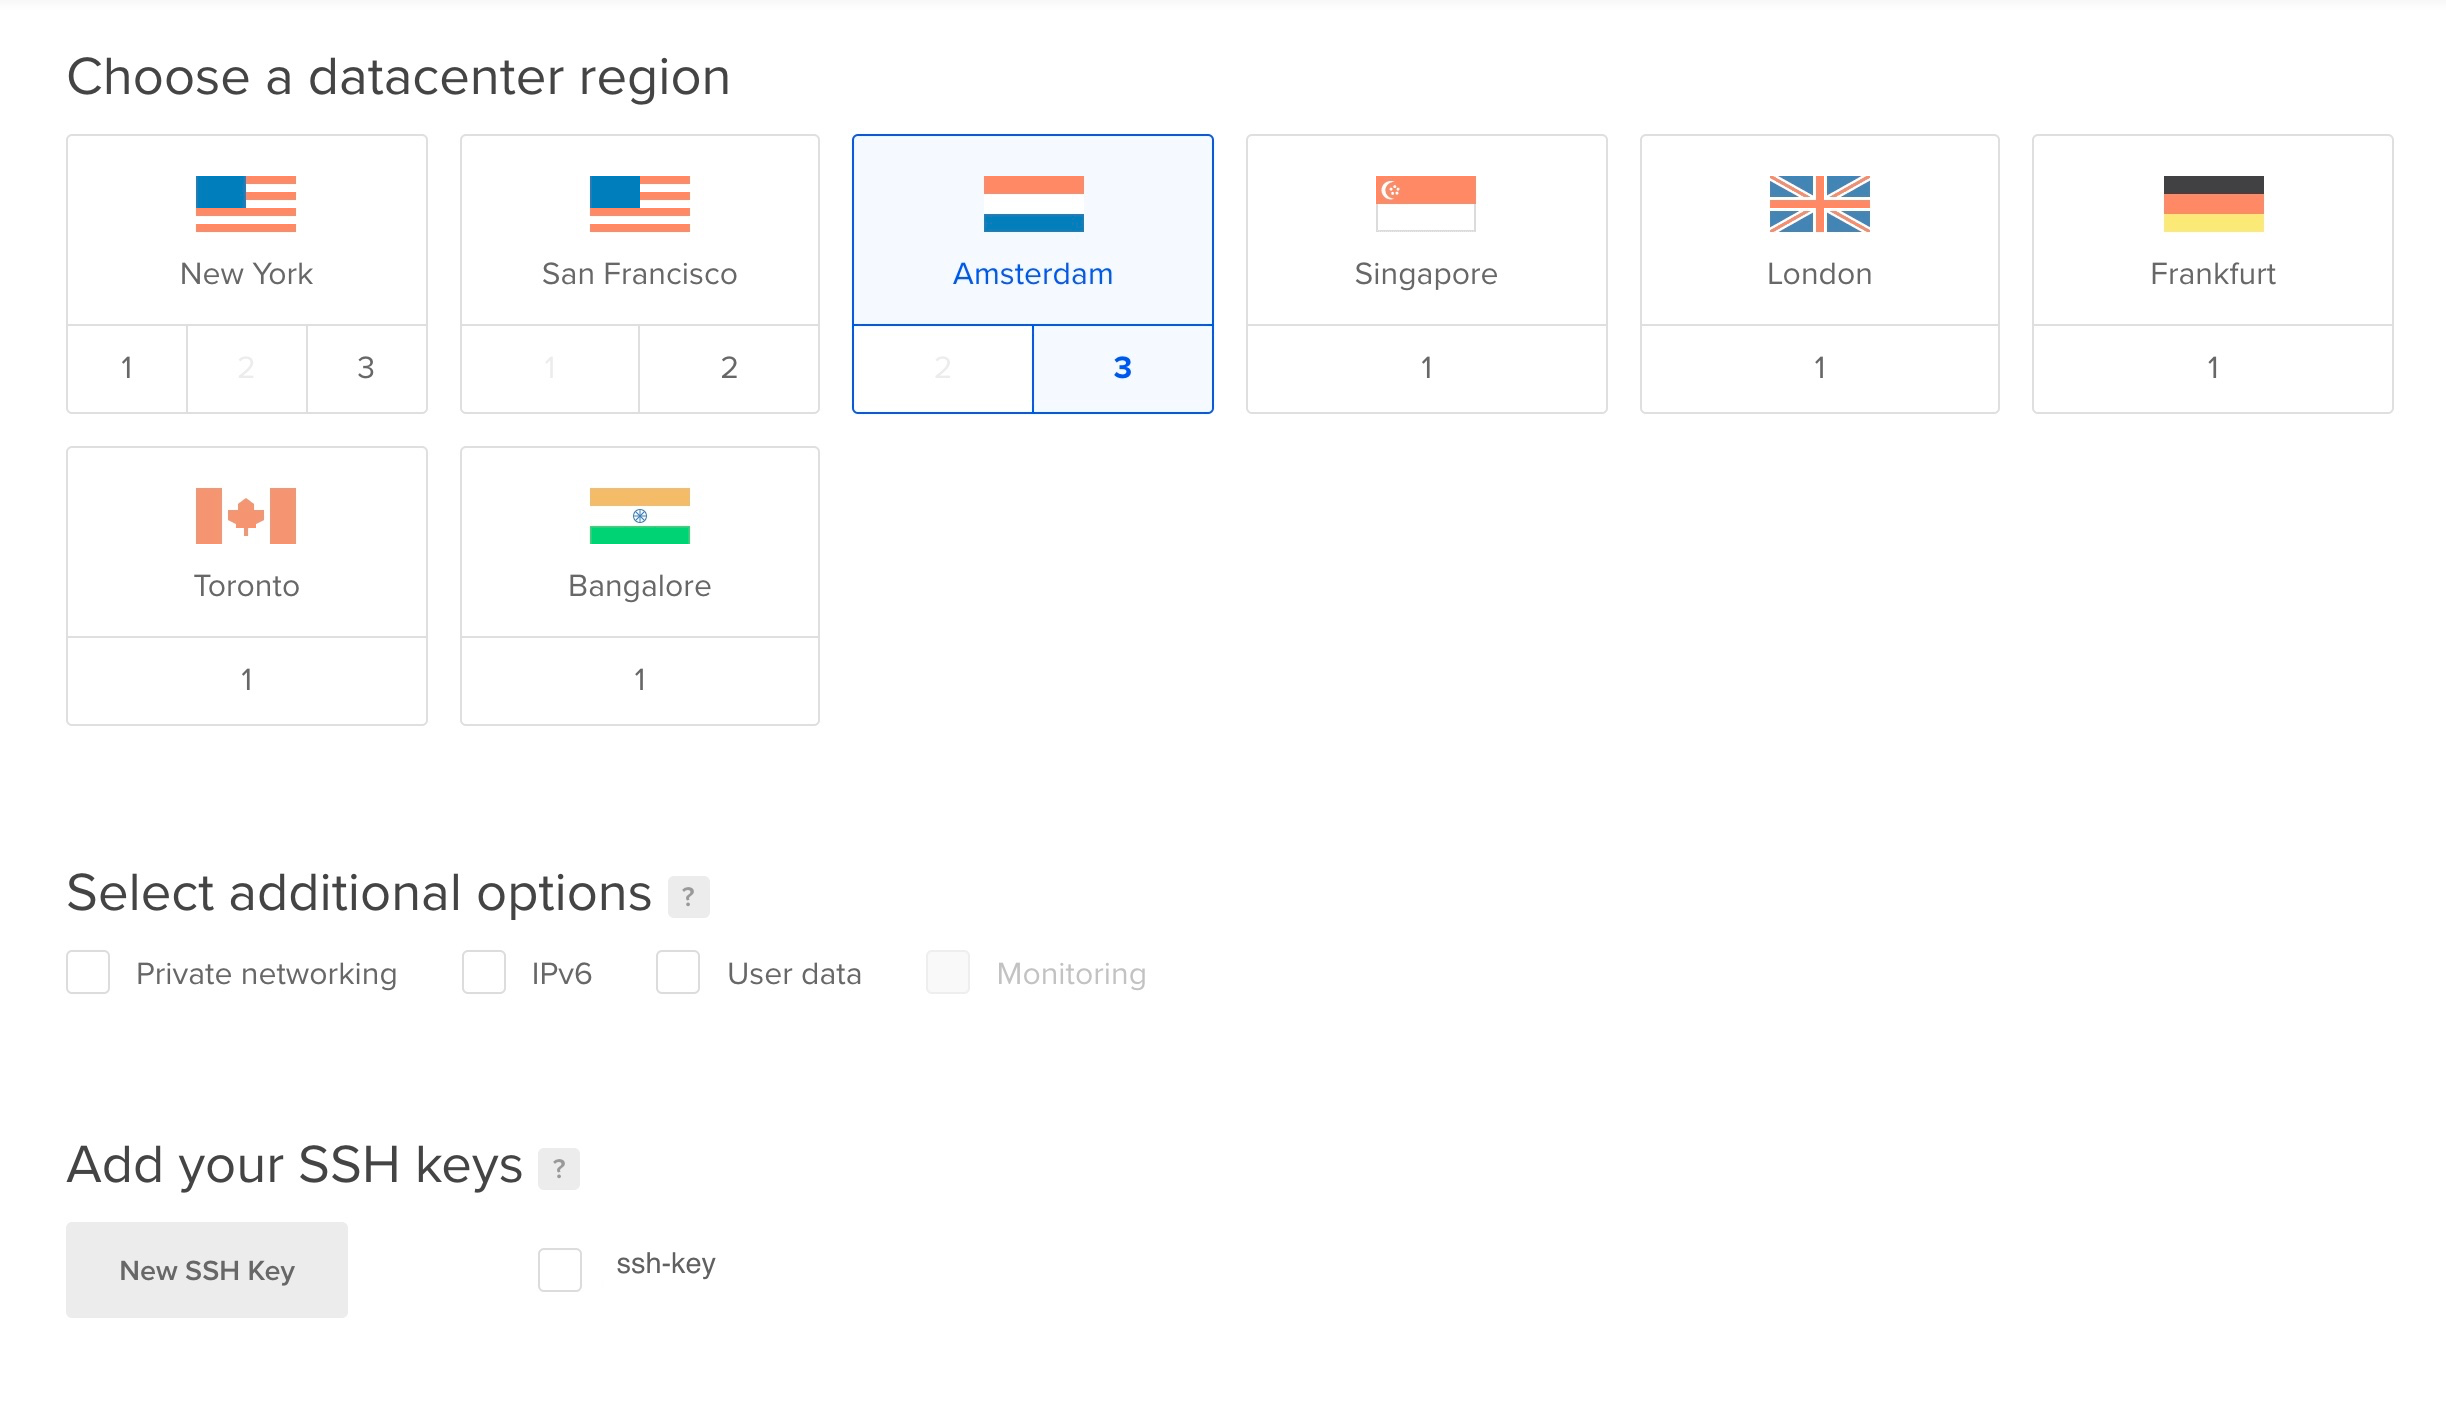
\includegraphics[scale=0.15]{slike/lokacijaIssh}
        \caption{Odabir lokacije i ssh ključeva}
    \end{figure}

    Kako sada prvi puta pristupamo poslužitelju jedini korisnik
    koji postoji je root. Root je korisnik na unixoidima koji može izvršiti
    svaku naredbu i pristupiti svakoj datoteci. Njemu pristupamo naredbom \\
    
    \noindent
    \code{\$ ssh root@139.59.159.111} \\

    Kada smo se prijavili na poslužitelja prvu stavr koju moramo napraviti je
    ažurirati sustav. To ćemo napraviti koristeći FreeBSD-ov upravitelj
    paketima \code{pkg} i njegove naredbe \code{update} i \code{upgrade}. \\

    \noindent
    \code{\# pkg update} \\
    \code{\# pkg upgrade} \\

    Sada možemo instalirati OpenVPN. \\

    \noindent
    \code{\# pkg install openvpn} \\

    Konfiguracijske datoteke ćemo smjestiti u direktorij
    \code{/usr/local/etc/openvpn} koji prvo moramo stvoriti. \\

    \noindent
    \code{\# mkdir /usr/local/etc/openvpn} \\

    \noindent
    Openvpn nudi predloške konfiguracijskih datoteka stoga ćemo kopirati
    predložak za konfiguraciju poslužitelja u naš direktorij

    \noindent
    \code{\# cp
    /usr/local/share/examples/openvpn/sample-config-files/server.conf
    \textbackslash} \\
    \code{\-\ \-\ \-\ \-\ \-\ /usr/local/etc/openvpn/openvpn.conf}

    \subsubsection{Konfiguracija}
        Kako bi mogli zaštititi našu vezu potrebno je šifrirati sav promet
        između poslužitelja i klijenta i osigurati inegritet svake poruke.
        Za šifriranje podataka ćemo koristiti simetrično šifriranje zbog svoje
        brzine, a za to nam je potreban simetrični ključ odnsno više ukoliko
        netko uspije dešifrirati jednu od naših poruka. Kako bi osigurali
        integritet poruka potrebno ih je potpisati i omogućiti provjeru
        potpisa. Ovaj problem ćemo rješiti digitalnim certifikatima koje ćemo
        sami napraviti. OpenVPN dolazi sa alatom Easy-RSA koji će nam poslužiti za izgradnju
        infrastrukture javnog ključa (\textit{engl. PKI - public key
        infrastructure}). PKI služi kako bi se javni ključevi povezali s
        pripadajućim osobama ili oragnizacijama. Proces povezivanja izvršava
        tijelo za certificiranje (\textit{engl. CA - certification authority}.
        CA također potvrđuje pripada li javni ključ osobi navedenoj u
        certifikatu. U praksi se CA nalazi na posebnom računalu, ali kako ovo
        radimo za privatnu uporabu naš CA će se nalaziti na poslužitelju.

        Kako je Easy-RSA omotač oko složene programske knjižnice OpenSSL ona
        nam je jedini preduvjet te ćemo ju instalirati naredbom \\

        \noindent
        \code{\# pkg install openssl} \\

        Nakon toga ćemo kopirati \code{easy-rsa} direktorij u naš direktorij sa svom
        konfiguracijom. \\

        \noindent
        \code{\# cp -r /usr/local/share/easy-rsa
        /usr/local/etc/openvpn/easy-rsa} \\

        Sada ćemo se premjestiti u Easy-RSA direktoriji i urediti njegovu
        konfiguracijusku datoteku \code{vars}. \\

        \noindent
        \code{\# cd /usr/local/etc/openvpn/easy-rsa} \\
        \code{\# vim vars} \\

        U nastavku su navedena polja koja je potrebno izmjeniti:
        
        \noindent
        \code{set\_var EASYRSA\_REQ\_COUNTRY   \-\ "<ZEMLJA>"} \\
        \code{set\_var EASYRSA\_REQ\_PROVINCE  "<ZUPANIJA>"} \\
        \code{set\_var EASYRSA\_REQ\_CITY      \-\ \-\ \-\ \-\ "<GRAD>"} \\
        \code{set\_var EASYRSA\_REQ\_ORG       \-\ \-\ \-\ \-\ \-\ "<ORGANIZACIJA>"} \\
        \code{set\_var EASYRSA\_REQ\_EMAIL     \-\ \-\ \-\ "<EMAIL>"} \\
        \code{set\_var EASYRSA\_REQ\_OU        \-\ \-\ \-\ \-\ \-\ \-\  "<ORGANIZACIJSKA JEDINICA>"} \\
        \code{set\_var EASYRSA\_KEY\_SIZE      \-\ \-\ \-\ \-\ <broj> \# duljina rsa ključa u
        bitovima} \\
        \code{set\_var EASYRSA\_CA\_EXPIRE     \-\ \-\ \-\ <broj> \# trajanje CA ključa u
        danima} \\
        \code{set\_var EASYRSA\_CERT\_EXPIRE   \-\ <broj> \# trajanje certifikata u
        danima} \\

        Kako je \code{easy-rsa} skripta pisana za ljusku sh, dok
        FreeBSD koristi csh potrebno je naredbom \code{sh} 
        pokrenuti sh ljsuksu. Sada možemo inicijalizirati PKI \\

        \code{\# ./easy-rsa.real init-pki} \\
        
        \begin{figure}[H]
            \centering
            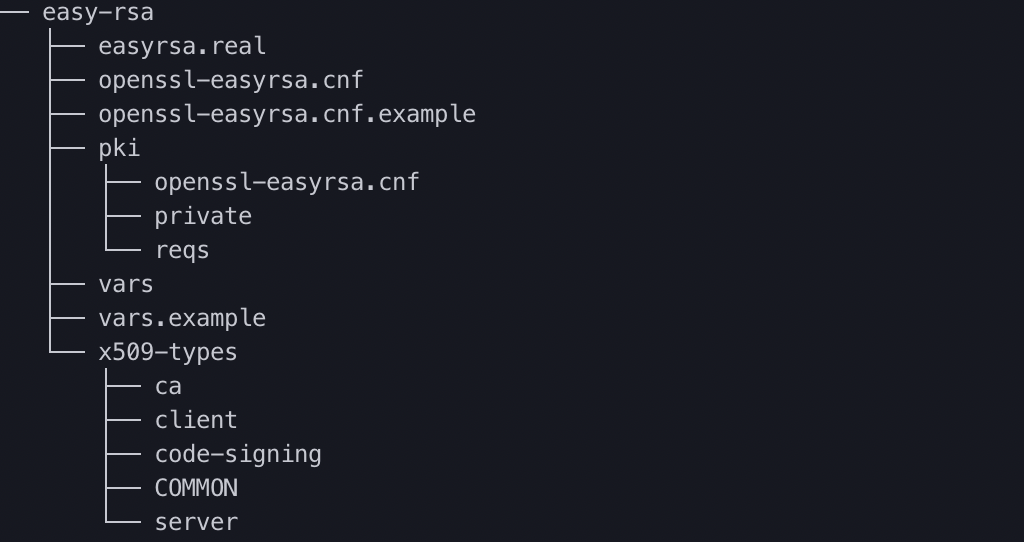
\includegraphics[scale=0.5]{slike/afterPkiInit}
            \caption{Struktura direktorija nakon inicijalizacije PKI}
        \end{figure}
        
        \noindent
        nakon čega ćemo stvoriti CA  \\

        \noindent
        \code{\# ./easy-rsa.real build-ca} \\
        
        \begin{figure}[H]
            \centering
            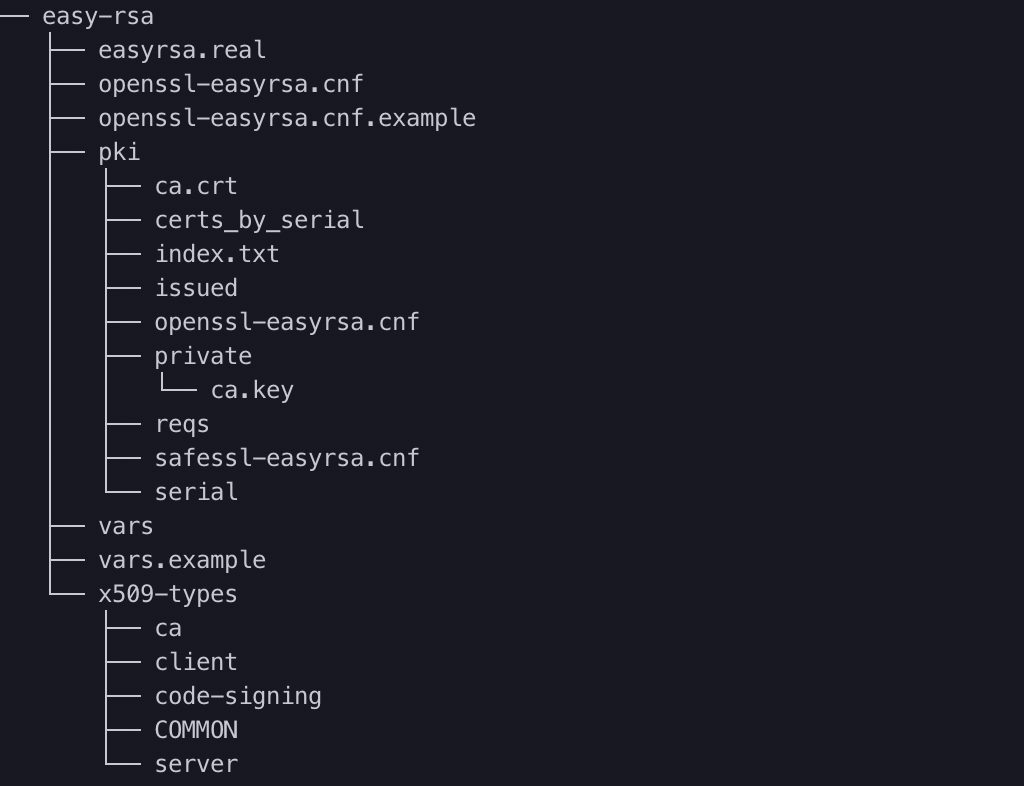
\includegraphics[scale=0.5]{slike/afterBuildCa}
            \caption{Struktura direktorija nakon stvaranja korjenskog
            certifikata}
        \end{figure}

        \noindent
        Ovom naredbom smo stvorili par ključeva koji ćemo koristiti za
        potpisivanje izdanih certifikata. 

        \noindent
        Sada ćemo generirati serverov certifikat naredbom \\

        \noindent
        \code{\# ./easy-rsa.real build-server-full <ime-server> nopass } \\

        \noindent
        gdje je \code{<ime-server>} ime certifikata, a s \code{nopass} opcijom ćemo
        generirati nešifrirani ključ kako bi mogli automatski pokrenuti OpenVPN
        uslugu prilikom pokretanja sustava bez upisivanja lozinke ključa.

        Na sličan način ćemo generirati klijentove certifikate \\

        \noindent
        \code{\# ./easy-rsa.real build-client-full <ime-klijent> nopass} \\
        
        \begin{figure}[H]
            \centering
            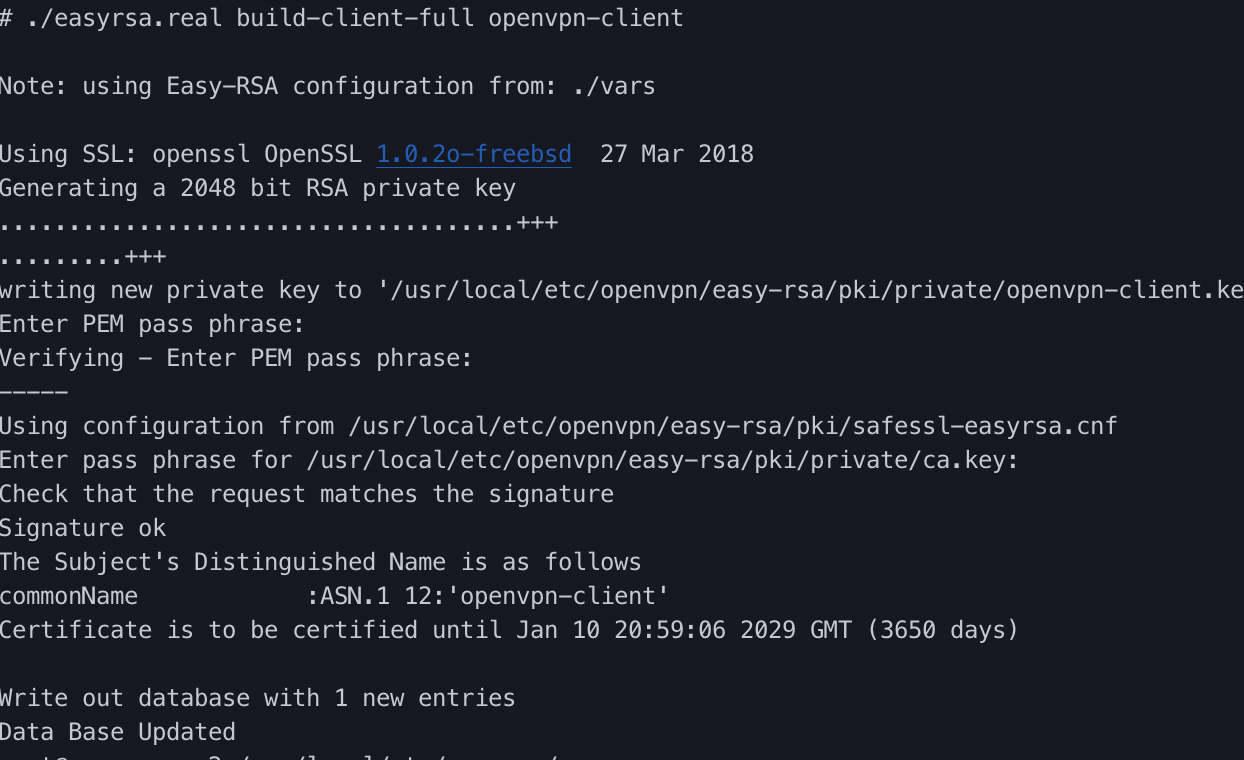
\includegraphics[scale=0.5]{slike/buildClientCert}
            \caption{Stvaranje certifikata}
        \end{figure}

        \begin{figure}[H]
            \centering
            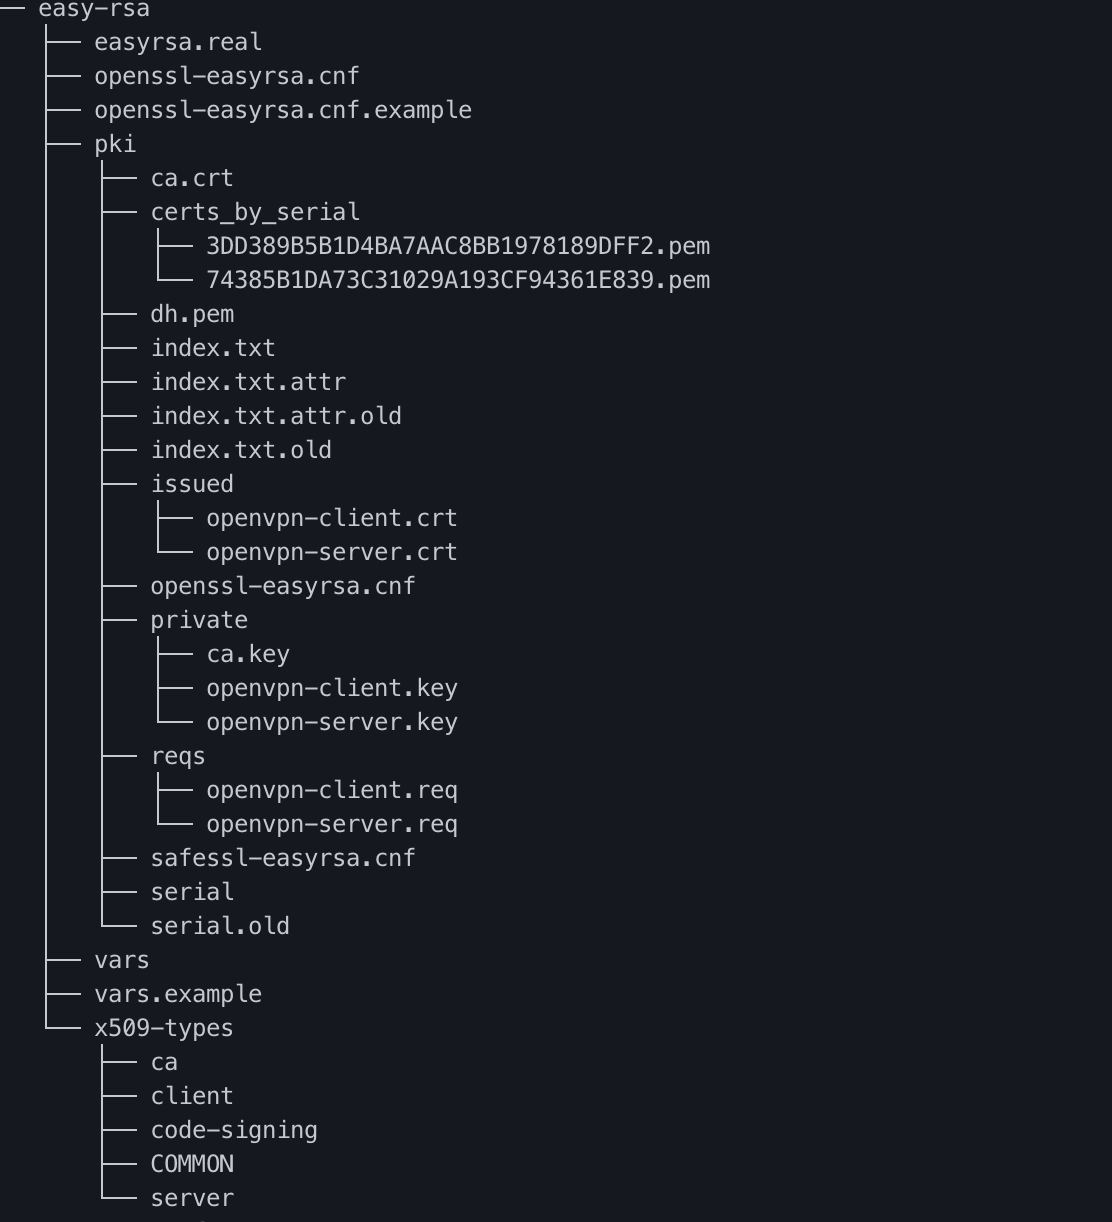
\includegraphics[scale=0.5]{slike/afterClientAndServerCert}
            \caption{Struktura direktorija nakon stvaranja klijentskog i
            poslužiteljevog certifikata}
        \end{figure}

        \noindent
        Za šifriranje same poruke koristit ćemo simetričan ključ generiran
        Diffie-Hellman razmjenom. Za to su nam potrebni Diffie-Hellman
        parametri koje stvaramo naredbom \\

        \noindent
        \code{\# ./easyrsa.real gen-dh} \\

        \noindent
        Do sada smo sve naredbe izvršavali na poslužitelju te smo generirali
        velik broj datoteka od kojih ćemo neke morati premjestiti na klijentsko
        računalo. Kako bi znali koje datoteke premejstiti potrebno je razumjeti
        čemu svaka od njih služi. Sve su datoteke stvorene u
        \code{easy-rsa/pki/} 
        direktoriju pa ćemo se u njega pozicionirati. \\

        \begin{itemize}
        \item \code{ca.crt} - certifikat koji se koristi za validaciju ostalih
        certifikata, potrebno ga je kopirati na poslužitelja i sve klijente
        \item \code{ca.key} - ključ koji CA koristi za izdavanje certifikata
        \item \code{reqs/} - direktorij koji sadrži zahtjeve za izdajom
        certifikata 
        \item \code{issued/<ime-server>.crt} - certifikat servera koji služi za
        provjeru potpisa na poruci, potrebno ga je prebaciti na poslužitelja
        \item \code{private/<ime-server>.key} - privatni ključ polužitelja
        koji se koristi za potpisivanje poruke, potrebno ga je prebaciti na
        poslužitelja
        \item \code{issued/<ime-klijent>.crt} - certifikat klijenta koji služi za
        provjeru potpisa na poruci, potrebno ga je prebaciti na klijentsko
        računalo
        \item \code{private/<ime-klijent>.key} - privatni ključ klijenta
        koji se koristi za potpisivanje poruke, potrebno ga je prebaciti na
        klijentsko računalo
        \item \code{dh.pem} - Diffie Hellman parametri, potrebno ih je prebaciti na
        poslužitelja
        \end{itemize}

        \noindent
        Ključeve poslužitelja ćemo premjestiti u poseban direktorij \\

        \noindent
        \code{\# mkdir /usr/local/etc/openvpn/keys} \\
        \code{\# cp pki/dh.pem \textbackslash} \\
        \code{\-\ \-\ \-\ \-\ \-\ pki/ca.crt \textbackslash} \\
        \code{\-\ \-\ \-\ \-\ \-\ pki/issued/<ime-server>.crt \textbackslash} \\
        \code{\-\ \-\ \-\ \-\ \-\ pki/private/<ime-server>.key \textbackslash} \\
        \code{\-\ \-\ \-\ \-\ \-\ /usr/local/etc/openvpn/keys} \\

        \begin{figure}[H]
            \centering
            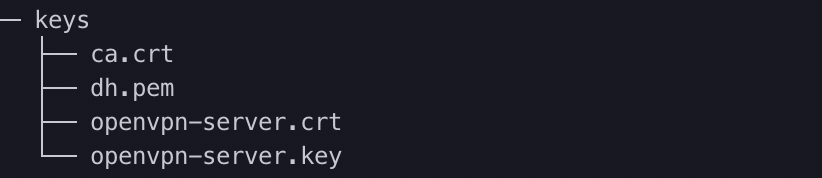
\includegraphics[scale=0.7]{slike/serverKeys}
            \caption{Sadržaj \code{keys} direktorija na poslužitelju}
        \end{figure}

        \noindent
        Prije nego što počnemo konfigurirati klijentsko računalo, potrebno je u
        konfiguraciji poslužitelja navesti putanje do certifikata, ključeva i 
        parametara. To ćemo napraviti u datoteci \code{openvpn.conf} koju smo
        na samom početku kopirali u \code{/usr/local/etc/openvpn}. \\
        
        \noindent
        \code{\# vim /usr/local/etc/openvpn/openvpn.conf} \\
        
        \noindent
        Potrebno je urediti sljedeće linije \\

        \noindent
        \code{ca /usr/local/etc/openvpn/keys/ca.crt} \\
        \code{cert /usr/local/etc/openvpn/keys/<ime-server>.crt} \\
        \code{key /usr/local/etc/openvpn/keys/<ime-server>.key} \\
        \code{dh /usr/local/etc/openvpn/keys/dh.pem} \\ 

        \begin{figure}[H]
            \centering
            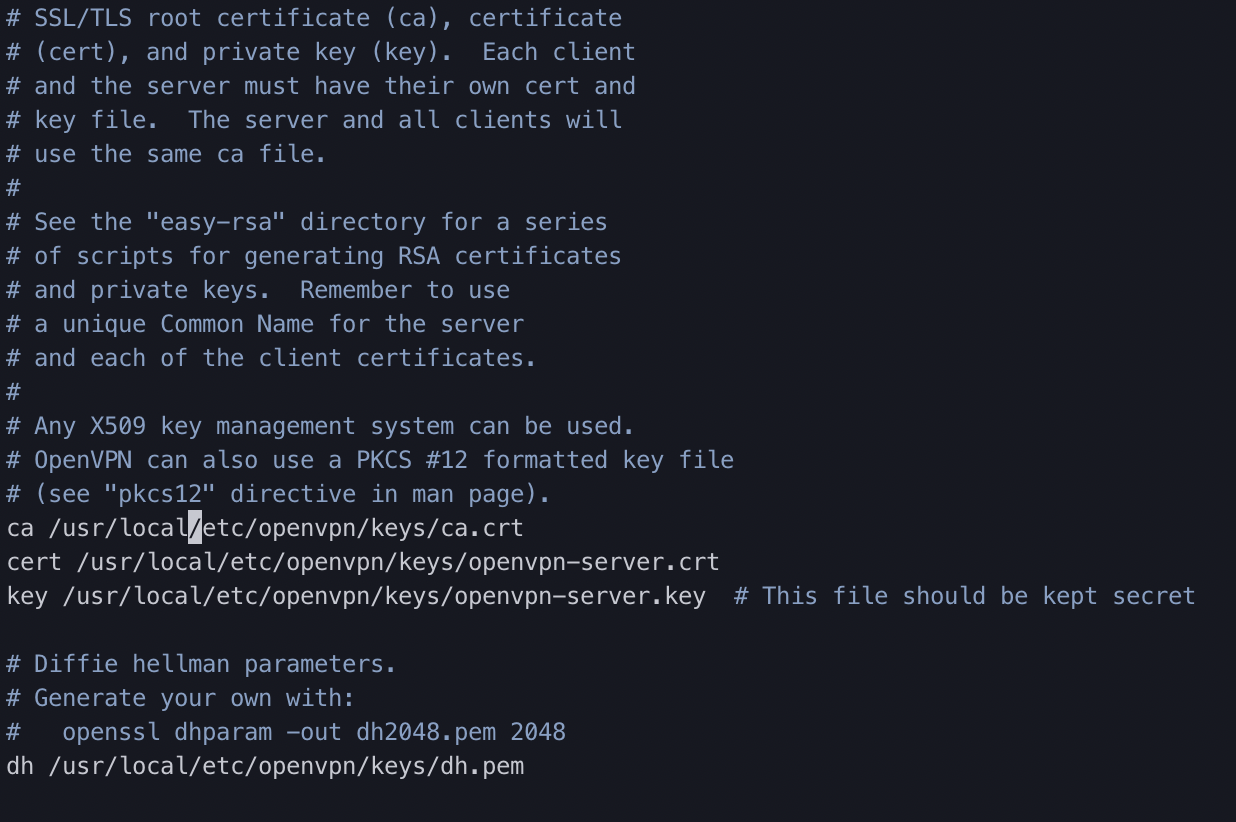
\includegraphics[scale=0.57]{slike/serverPaths}
            \caption{Putanje do ključeva i certifikata u datoteci
            \code{openvpn.conf}}
        \end{figure}
        
        Sada možemo postaviti klijentsko računalo. Kako smo već pripremili
        većinu klijentovih datoteka na poslužitelju, potrebno ih je kopirati.
        Radi se o osjetljivim datotekama stoga nam je potreban siguran način
        slanja datoteka preko mreže za što ćemo koristiti program
        \textit{secure copy}. Nakon što instaliramo openvpn isto kao i na
        poslužiteljskom računalu možemo kopirati predložak konfiguracije \\

        \noindent
        \code{\# cp
        /usr/local/share/examles/openvpn/sample-config-files/client.config
        \textbackslash} \\
        \code{\-\ \-\ \-\ \-\ \-\ /usr/local/etc/openvpn/openvpn.conf} \\

        \noindent
        Također stvorit ćemo direktorij u koji ćemo spremiti ključeve i
        certifikate \\

        \noindent
        \code{\# mkdir /usr/local/etc/openvpn/keys}\\

        \noindent
        Sada možemo kopirati potrebne datoteke sa poslužitelja \\

        \noindent
        \code{\$ scp
        root@<ip-server>:/usr/local/etc/openvpn/easy-rsa/pki/ca.crt keys } \\
        \code{\$ scp
        root@<ip-server>:\textbackslash} \\
        \code{\-\
        \-\ \-\ \-\ \-\ \-\ /usr/local/etc/openvpn/easy-rsa/pki/issued/<ime-klijent>.crt
        \textbackslash} \\
        \code{\-\ \-\ \-\ \-\ \-\ \-\ keys} \\
        \code{\$ scp
        root@<ip-server>:\textbackslash} \\
        \code{\-\
        \-\ \-\ \-\ \-\ \-\
        /usr/local/etc/openvpn/easy-rsa/pki/private/<ime-klijent>.key
        \textbackslash} \\
        \code{\-\ \-\ \-\ \-\ \-\ \-\ keys} \\

        \begin{figure}[H]
            \centering
            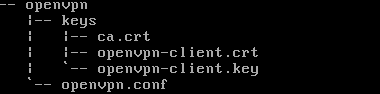
\includegraphics[scale=0.7]{slike/clientKeys}
            \caption{Sadržaj \code{keys} direktorija na klijentu}
        \end{figure}

        \noindent
        U konfiguraciji (\code{openvpn.conf}) osim putanja do certifikata i
        ključeva potrebno je unjeti ip adresu poslužitelja \\

        \noindent
        \code{remote <ip-server> 1194} \\
        \code{ca /usr/local/etc/openvpn/keys/ca.crt} \\
        \code{cert /usr/local/etc/openvpn/keys/<ime-server>.crt} \\
        \code{key /usr/local/etc/openvpn/keys/<ime-server>.key} \\

        Za upravljanje servisima koristimo naredbu \code{service}. Prvo ćemo
        njome pokrenuti OpenVPN servis na poslužitelju i nakon toga na klijentu

        \noindent
        \code{\# service openvpn run} \\

        \noindent
        Sada možemo alatom \code{ifconfig} provjeriti stanje mrežnih sučelja \\
        na klijentu: \\
        \begin{figure}[H]
            \centering
            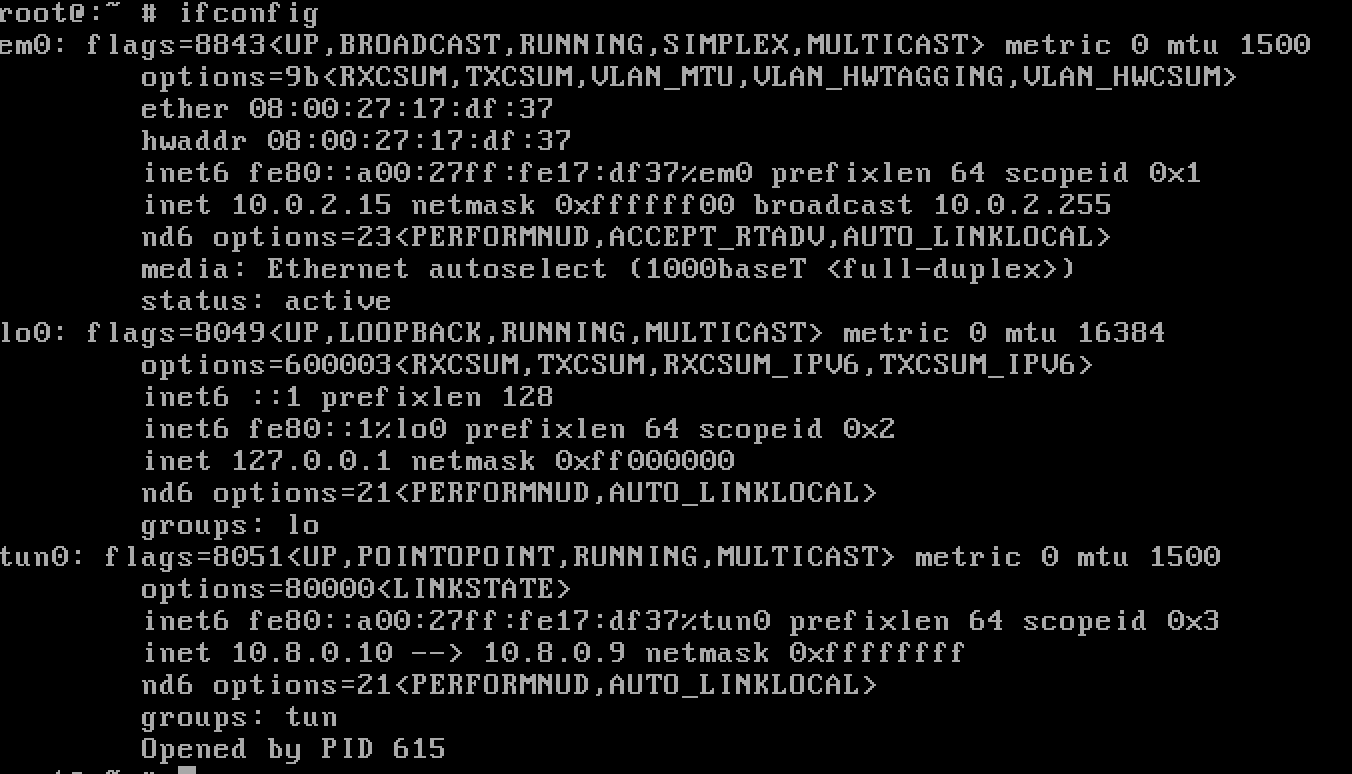
\includegraphics[scale=0.5]{slike/clientIfconfig}
            \caption{Mrežna sučelja klijenta }
        \end{figure}
        na poslužitelju: \\
        \begin{figure}[H]
            \centering
            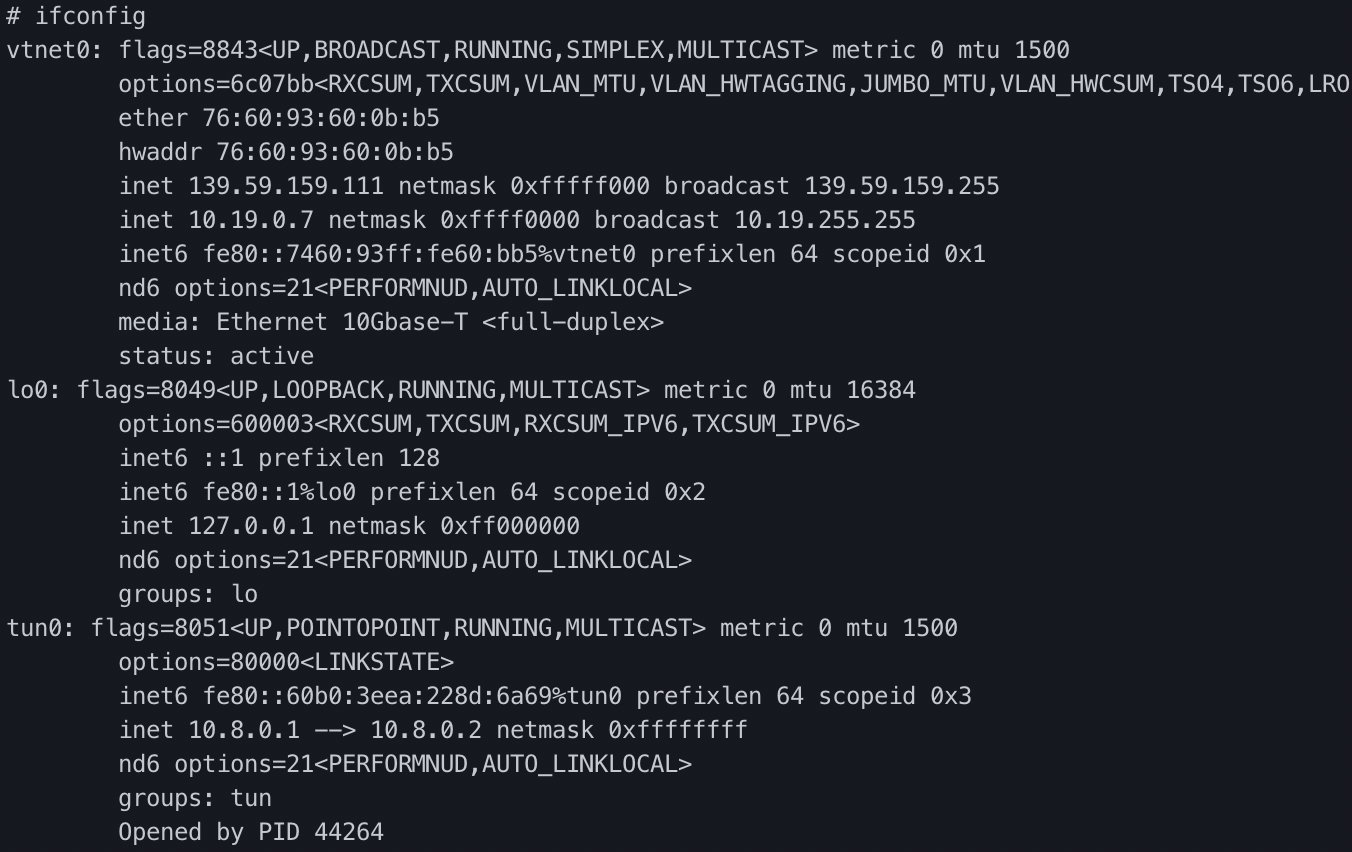
\includegraphics[scale=0.5]{slike/serverIfconfig}
            \caption{Mrežna sučelja poslužitelja}
        \end{figure}

        Možemo uočiti novo sučelje \code{tun0} koje predstavlja virtualno
        sučelje mrežnog sloja. Izvršavanjem naredbe \code{ping} možemo provjeriti je
        li klijentsko računalo stvarno povezano s poslužiteljem. \\

        \noindent
        \code{\$ ping 10.8.0.1} \\

        Kako nam je cilj povezati dva klijenta koji se nalaze u različitim
        privatnim mrežama na isti ćemo pripremiti još jednog klijenta. Njegova
        konfiguracija će biti jednaka konfiguraciji prvog klijenta, a izlaz
        naredbe \code{ifconfig}:
        \begin{figure}[H]
            \centering
            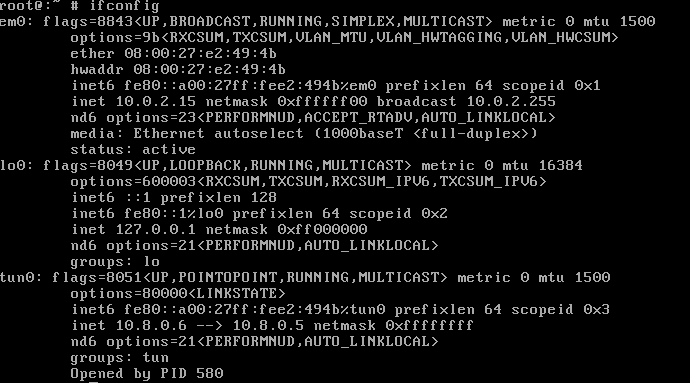
\includegraphics[scale=0.45]{slike/client2Ifconfig}
            \caption{Mrežna sučelja drugog klijenta}
        \end{figure}

        \noindent
        Ako sada pokušamo naredbom
        \code{\$ ping 10.8.0.6}
        provjeriti jesu li klijenti međusobno povezani nećemo dobiti nikakav
        rezultat. Razlog tome je što pretpostavljena konfiguracija poslužitelja
        ne dozvoljava komunikaciju između klijenata. Kako bi to omogućili
        potrebno je u konfiguracijskoj datoteci poslužitalja otkomentirati liniju 

        \noindent 
        \code{client-to-client} \\

        \noindent
        Sada ćemo ponovo pokrenuti OpenVPN i ispitati jesu li klijenti
        međusobno povezani \\

        \noindent
        \code{\# service openvpn restart} \\
        \code{\$ ping 10.8.0.6} \\
        \begin{figure}[H]
            \centering
            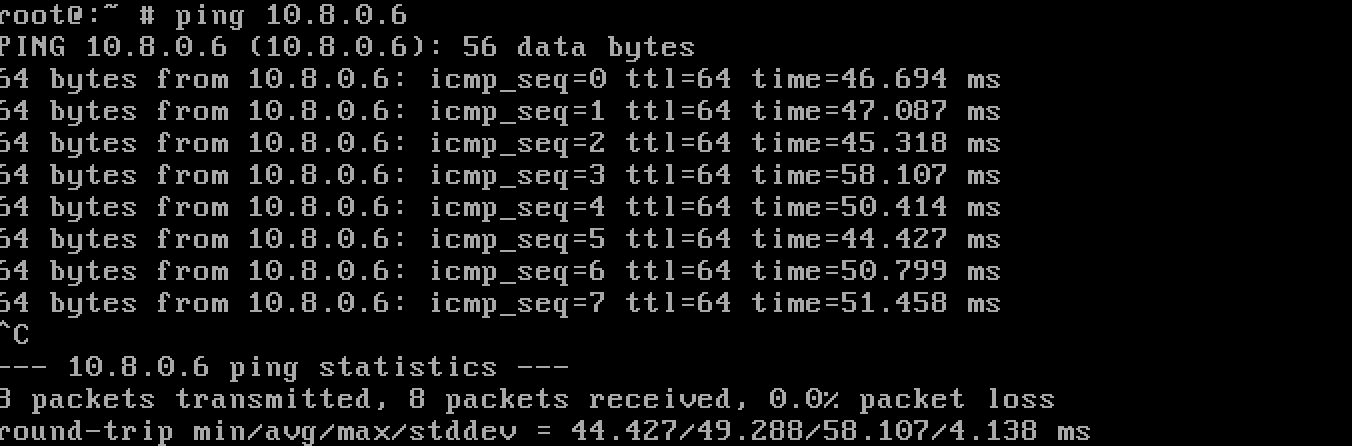
\includegraphics[scale=0.5]{slike/pingResult}
            \caption{Izlaz naredbe ping}
        \end{figure}

        Za kraj možemo pokušati kopirati datoteku s jednog klijenta na drugi
        koristeći \code{tun0} sučelja. Na klijentu s adresom \code{10.8.0.6}
        stvorit ćemo datoteku \code{pozdrav.txt} i u nju nešto zapisati \\ 

        \noindent
        \code{\$ touch pozdrav.txt} \\
        \code{\$ echo "Bok" > pozdrav.txt} \\

        \noindent
        Sada ćemo sa drugog klijenta (adresa \code{10.8.0.10}) kopirati
        \code{pozdrav.txt} datoteku i ispistai ju \\
        \code{\$ scp root@10.8.0.6:/root/pozdrav.txt .} \\
        \code{\$ cat /root/pozdrav.txt}\\

        \begin{figure}[H]
            \centering
            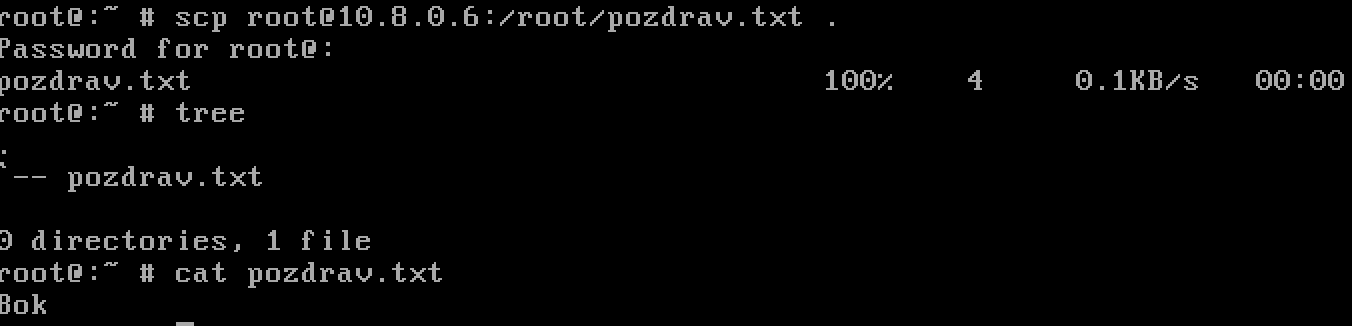
\includegraphics[scale=0.45]{slike/pozdrav}
            \caption{Kopiranje i ispis datoteke \code{pozdrav.txt}}
        \end{figure}
